\section{Bibliometric Analysis Methodology}\label{sec:Bibliometric-Methodology}

To justify the focus on graph-based approaches in traffic forecasting and to
trace the evolution of the field, we conducted a systematic bibliometric
analysis. This appendix supports the single motivating observation used in
the Introduction; it is not part of the forecasting experiments.

\subsection{Data Collection and Initial Filtering}

A broad search in Scopus with the keyword ``traffic forecast*'' retrieved
approximately $60{,}000$ documents. Filtering for peer-reviewed English
articles in Engineering or Computer Science yielded a core collection of
$784$ articles published between $2000$ and $2025$.

\subsection{Keyword Processing and Semantic Clustering}

The raw data contained $6{,}343$ unique keywords. After removing terms with
fewer than $10$ occurrences, $217$ keywords remained. An initial VOSviewer
network (Figure~\ref{fig:scopus-all}) showed near-duplicate terms
(``graph neural network'', ``GNN'', ``graph convolution network'') as
separate nodes.

\begin{figure}[!t]
\centering
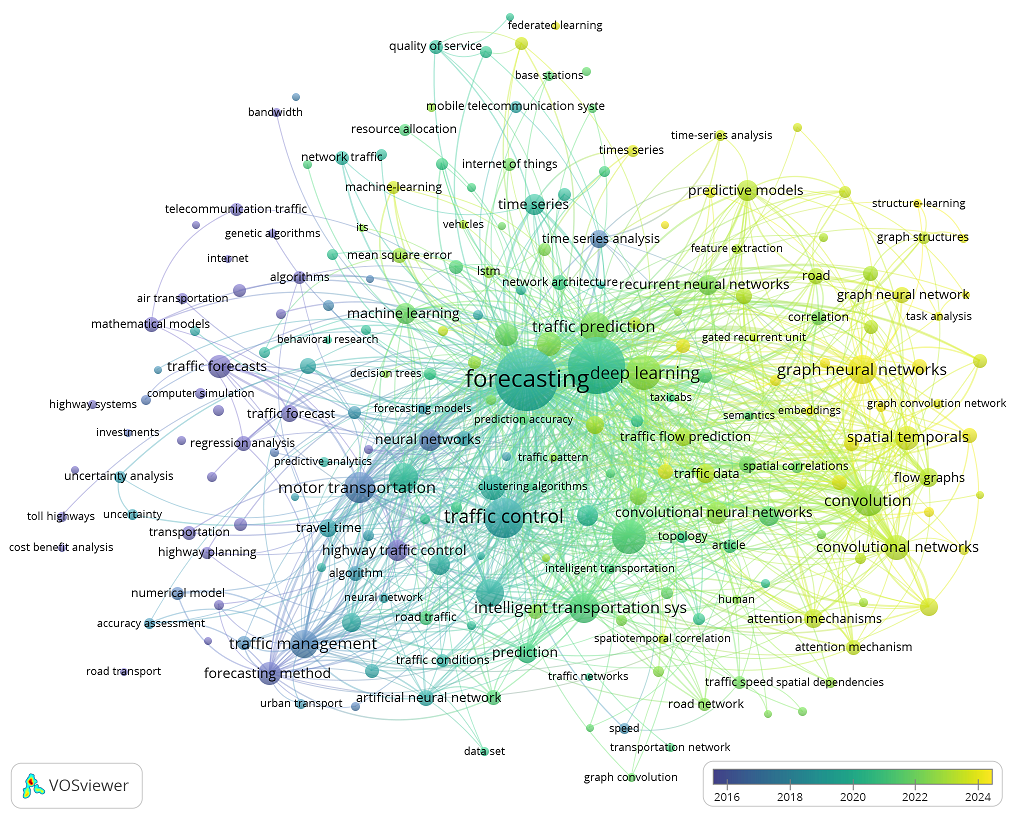
\includegraphics[width=1\linewidth]{scopus-all.png}
\caption{Initial keyword co-occurrence network ($217$ keywords) before
semantic grouping.}
\label{fig:scopus-all}
\end{figure}

A cleaning pipeline in the project repository (preprocessing, expansion of
$30$ common abbreviations, and Sentence-BERT semantic clustering) condensed
these terms into $66$ concept groups. Figure~\ref{fig:word-clouds} shows
word clouds for three representative clusters.

\begin{figure}[t]
    \centering
    \begin{subfigure}{0.32\textwidth}
        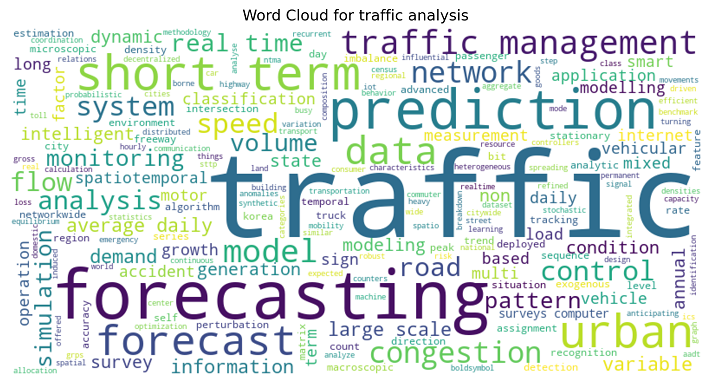
\includegraphics[width=\linewidth]{1-traffic analysis.png}
        \caption{Traffic analysis}
    \end{subfigure}
    \hfill
    \begin{subfigure}{0.32\textwidth}
        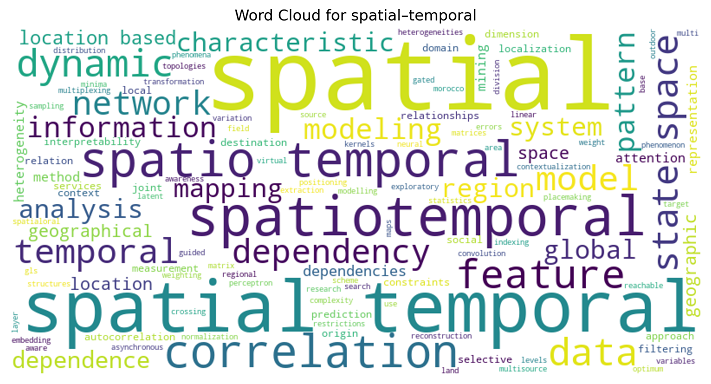
\includegraphics[width=\linewidth]{5-spatial–temporal.png}
        \caption{Spatio-temporal}
    \end{subfigure}
    \hfill
    \begin{subfigure}{0.32\textwidth}
        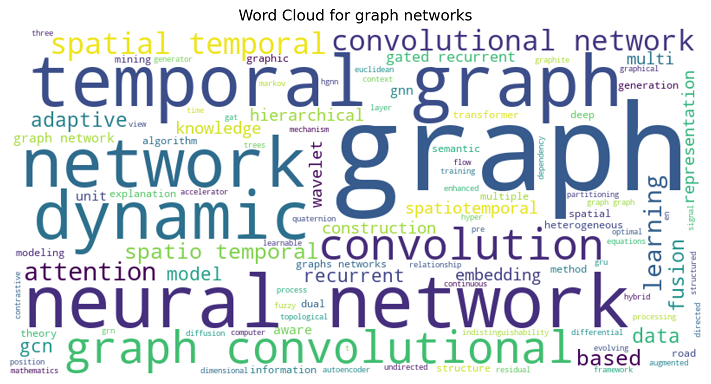
\includegraphics[width=\linewidth]{8-graph networks.png}
        \caption{Graph networks}
    \end{subfigure}
    \caption{Word clouds for three bibliometric clusters.}
    \label{fig:word-clouds}
\end{figure}

\subsection{Key Findings}

The refined network (Figure~\ref{fig:clustered_keywords}) shows that
graph-based methods are the most recent methodological focus in this
literature, while many such methods still rely on predefined graph
structures. That observation motivates studying graph structure learning
for traffic forecasting.

\begin{figure}[t]
\centering
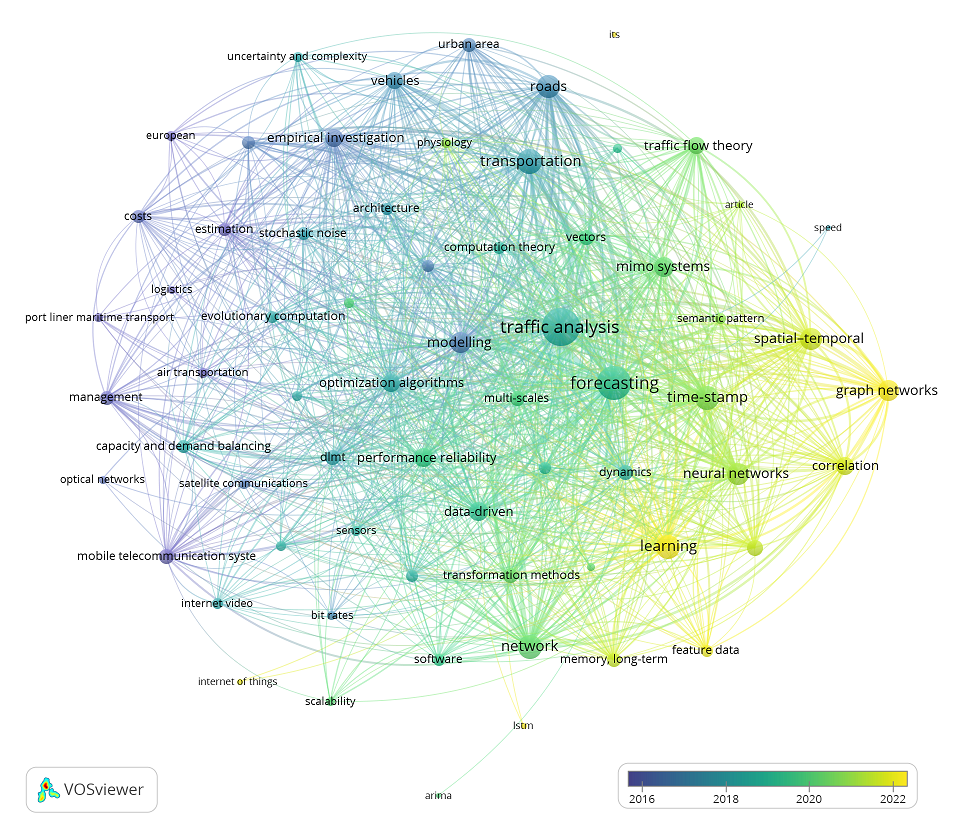
\includegraphics[width=.9\linewidth]{scopus-clustered.png}
\caption{Clustered keyword co-occurrence network from $784$ traffic
forecasting articles ($2000$--$2025$), colored by average publication year.}
\label{fig:clustered_keywords}
\end{figure}
